\chapter{Méthodes du gradient conjugué non linéaire}

\section{Introduction}

\textbf{Idée :} Adapter le gradient conjugué linéaire (efficace pour les problèmes quadratiques) aux fonctions objectives non linéaires générales.

\section{Méthode de Fletcher et Reeves}

Fletcher et Reeves \cite{fletcher1964function} ont proposé deux changements majeurs par rapport à l'algorithme linéaire pour minimiser une fonction $f$ quelconque.

\subsection{1. Recherche linéaire (Line Search)}
Contrairement au cas quadratique où le pas $\alpha_k$ est donné par une formule exacte, ici on substitue la formule :
\[
\alpha_k = \frac{r_k^\top r_k}{p_k^\top A p_k}
\]
par une \textbf{recherche linéaire} pour approximer le minimum de $f$ le long de la direction $p_k$.

\subsection{2. Substitution du résidu par le gradient}
Dans le cas linéaire, le résidu $r_k$ correspondait au gradient de la fonction quadratique $\phi$. Pour le cas général, on substitue le gradient de $\phi$ par le gradient de $f$ :
\[
r_k = \nabla \phi(x_k) \longrightarrow \nabla f_k.
\]

\subsection{Formule du \texorpdfstring{$\beta_{FR}$}{beta\_FR}}
La formule pour $\beta$ utilisée dans le cas linéaire ($\beta = \frac{r_{k+1}^\top r_{k+1}}{r_k^\top r_k}$) devient la formule de Fletcher-Reeves :
\[
\boxed{\beta_{FR} = \frac{\nabla f_{k+1}^\top \nabla f_{k+1}}{\nabla f_k^\top \nabla f_k}}.
\]
Ceci définit l'Algorithme 9.

\begin{remarque}
Il n'y a pas de signe moins dans cette formule.
\end{remarque}

\begin{figure}[H]
\centering
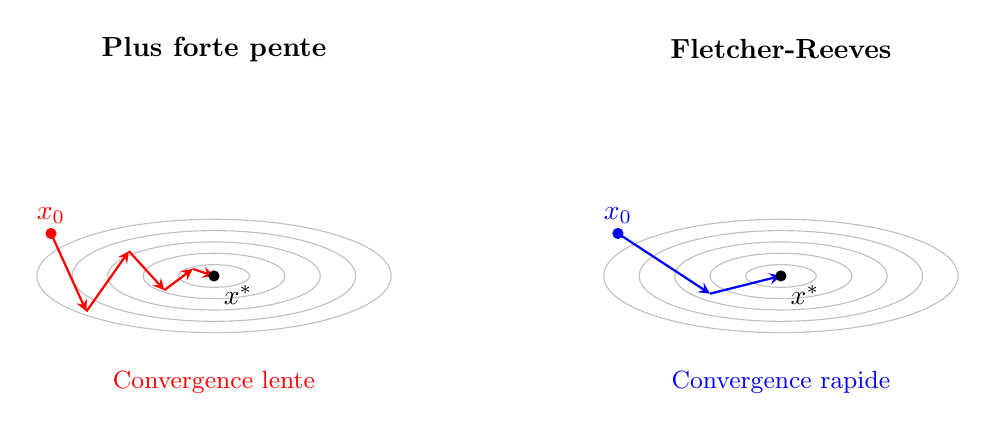
\begin{tikzpicture}[scale=0.9]
    % Left plot: Steepest Descent (zigzag)
    \begin{scope}[shift={(-4,0)}]
        \node at (0, 3.2) {\textbf{Plus forte pente}};
        
        % Draw elliptical contours
        \draw[gray!50] (0,0) ellipse (2.5cm and 0.8cm);
        \draw[gray!50] (0,0) ellipse (2.0cm and 0.64cm);
        \draw[gray!50] (0,0) ellipse (1.5cm and 0.48cm);
        \draw[gray!50] (0,0) ellipse (1.0cm and 0.32cm);
        \draw[gray!50] (0,0) ellipse (0.5cm and 0.16cm);
        
        % Steepest descent path (zigzag)
        \coordinate (sd0) at (-2.3, 0.6);
        \coordinate (sd1) at (-1.8, -0.5);
        \coordinate (sd2) at (-1.2, 0.35);
        \coordinate (sd3) at (-0.7, -0.2);
        \coordinate (sd4) at (-0.3, 0.1);
        \coordinate (sd5) at (0, 0);
        
        \draw[red, thick, -stealth] (sd0) -- (sd1);
        \draw[red, thick, -stealth] (sd1) -- (sd2);
        \draw[red, thick, -stealth] (sd2) -- (sd3);
        \draw[red, thick, -stealth] (sd3) -- (sd4);
        \draw[red, thick, -stealth] (sd4) -- (sd5);
        
        \filldraw[red] (sd0) circle (2pt) node[above] {$x_0$};
        \filldraw[black] (0,0) circle (2pt) node[below right] {$x^*$};
        
        \node[red] at (0, -1.5) {\small Convergence lente};
    \end{scope}
    
    % Right plot: Fletcher-Reeves (more direct)
    \begin{scope}[shift={(4,0)}]
        \node at (0, 3.2) {\textbf{Fletcher-Reeves}};
        
        % Draw elliptical contours
        \draw[gray!50] (0,0) ellipse (2.5cm and 0.8cm);
        \draw[gray!50] (0,0) ellipse (2.0cm and 0.64cm);
        \draw[gray!50] (0,0) ellipse (1.5cm and 0.48cm);
        \draw[gray!50] (0,0) ellipse (1.0cm and 0.32cm);
        \draw[gray!50] (0,0) ellipse (0.5cm and 0.16cm);
        
        % Fletcher-Reeves path (more direct, conjugate directions)
        \coordinate (fr0) at (-2.3, 0.6);
        \coordinate (fr1) at (-1.0, -0.25);
        \coordinate (fr2) at (0, 0);
        
        \draw[blue, thick, -stealth] (fr0) -- (fr1);
        \draw[blue, thick, -stealth] (fr1) -- (fr2);
        
        \filldraw[blue] (fr0) circle (2pt) node[above] {$x_0$};
        \filldraw[black] (0,0) circle (2pt) node[below right] {$x^*$};
        
        \node[blue] at (0, -1.5) {\small Convergence rapide};
    \end{scope}
\end{tikzpicture}
\caption{Comparaison de la plus forte pente (gauche) et Fletcher-Reeves (droite) sur des courbes de niveau elliptiques. La méthode de Fletcher-Reeves exploite les directions conjuguées pour converger plus rapidement.}
\label{fig:fr-vs-sd}
\end{figure}

\begin{figureexplanation}
La figure~\ref{fig:fr-vs-sd} illustre l'avantage du gradient conjugué non linéaire (Fletcher-Reeves) par rapport à la plus forte pente. Sur une fonction quadratique mal conditionnée (ellipses allongées), la plus forte pente zigzague en alternant entre directions orthogonales, tandis que Fletcher-Reeves exploite les directions conjuguées pour atteindre le minimum en moins d'itérations.
\end{figureexplanation}

\subsection{Illustration sur la fonction de Rosenbrock}

La \textbf{fonction de Rosenbrock} $f(x,y) = (1-x)^2 + 100(y-x^2)^2$ est un cas test classique pour les algorithmes d'optimisation. Elle possède un minimum unique en $(1,1)$ mais présente une vallée très étroite et courbée qui rend la convergence difficile.

\begin{figure}[H]
\centering

\includegraphics[width=0.85\textwidth]{1.png}
\caption{La fonction de Rosenbrock $f(x,y) = (1-x)^2 + 100(y-x^2)^2$, ayant un minimum unique en $(1,1)$.}
\label{fig:rosenbrock-surface}
\end{figure}

\begin{figureexplanation}
\textbf{Points clés à observer :}
\begin{itemize}
    \item \textbf{Forme de la surface :} La vallée parabolique (« banana valley ») est clairement visible. Le minimum global $(1,1)$ se trouve au fond de cette vallée étroite.
    \item \textbf{Échelle logarithmique :} L'axe vertical utilise $\log(Z)$ pour visualiser les grandes variations de la fonction.
    \item \textbf{Difficulté d'optimisation :} Atteindre le fond de la vallée est facile, mais progresser le long de la vallée vers le minimum est difficile pour de nombreuses méthodes.
\end{itemize}
\end{figureexplanation}

\begin{figure}[H]
\centering

\includegraphics[width=0.7\textwidth]{5.png}
\caption{Itérations de la méthode Fletcher-Reeves (gradient conjugué non linéaire) sur les courbes de niveau de la fonction de Rosenbrock.}
\label{fig:fletcher-reeves-rosenbrock}
\end{figure}

\begin{figureexplanation}
\textbf{Points clés à observer :}
\begin{itemize}
    \item \textbf{Trajectoire efficace :} La méthode converge vers le minimum $(1,1)$ en exploitant les directions conjuguées, sans utiliser explicitement la Hessienne.
    \item \textbf{Compromis :} Fletcher-Reeves offre une convergence plus rapide que la descente de gradient, tout en évitant le coût de calcul de la Hessienne (nécessaire pour Newton).
    \item \textbf{Adaptation au cas non-linéaire :} Bien que la théorie du gradient conjugué soit optimale pour les fonctions quadratiques, la méthode reste efficace sur cette fonction fortement non-quadratique.
\end{itemize}
\end{figureexplanation}

%%%%%%%%%%%%%%%%%%%%%%%%%%%%%%%%%%%%%%%%%%%%%%%%%%%%%%%%%%%%
\subsection{Propriété de descente globale}

Contrairement au cas quadratique, la direction $p_k$ générée par Fletcher-Reeves n'est pas automatiquement une direction de descente.

On a la relation :
\[
\nabla f_k^\top p_k = -\|\nabla f_k\|^2 + \beta_{FR} \nabla f_k^\top p_{k-1}.
\]
Si le second terme est grand, la direction peut remonter. Pour garantir la descente, il faut imposer des conditions strictes sur la recherche linéaire.

\begin{lemme}[Condition de descente]
Supposons que le pas $\alpha_k$ satisfait les \textbf{conditions de Wolfe fortes} avec un paramètre $0 < c_2 < \frac{1}{2}$.
Alors, la direction $p_k$ est toujours une direction de descente et satisfait l'encadrement suivant pour tout $k$ :
\[
-\frac{1}{1-c_2} \le \frac{\nabla f_k^\top p_k}{\|\nabla f_k\|^2} \le \frac{2c_2 - 1}{1-c_2}.
\]
\end{lemme}

\begin{proof}
\textbf{Préliminaire.} Considérons la fonction $t(\xi) = \frac{2\xi - 1}{1 - \xi}$.
Cette fonction est croissante sur $[0, \frac{1}{2}]$.
On a $t(0) = -1$ et $t(1/2) = 0$.
Comme $0 < c_2 < 1/2$, on a :
\[
-1 < \frac{2c_2 - 1}{1 - c_2} < 0.
\]

\textbf{Initialisation ($k=0$).}
On a $p_0 = -\nabla f_0$, donc $\nabla f_0^\top p_0 = -\|\nabla f_0\|^2$.
Le rapport vaut :
\[
\frac{\nabla f_0^\top p_0}{\|\nabla f_0\|^2} = -1.
\]
L'inégalité est satisfaite car :
\[
-\frac{1}{1-c_2} \le -1 < \frac{2c_2 - 1}{1 - c_2} \quad \text{(vérifié car } c_2 < 1/2 \text{)}.
\]

\textbf{Hérédité.} Supposons le résultat vrai pour $k$.
Calculons le rapport pour $k+1$ :
\[
\frac{\nabla f_{k+1}^\top p_{k+1}}{\|\nabla f_{k+1}\|^2} 
= \frac{\nabla f_{k+1}^\top (-\nabla f_{k+1} + \beta_{k+1}^{FR} p_k)}{\|\nabla f_{k+1}\|^2}
= -1 + \beta_{k+1}^{FR} \frac{\nabla f_{k+1}^\top p_k}{\|\nabla f_{k+1}\|^2}.
\]
En utilisant la définition de $\beta_{FR} = \frac{\|\nabla f_{k+1}\|^2}{\|\nabla f_k\|^2}$, on simplifie :
\[
\frac{\nabla f_{k+1}^\top p_{k+1}}{\|\nabla f_{k+1}\|^2} = -1 + \frac{\nabla f_{k+1}^\top p_k}{\|\nabla f_k\|^2}.
\]

La condition de courbure (seconde condition de Wolfe forte) impose :
\[
|\nabla f_{k+1}^\top p_k| \le c_2 |\nabla f_k^\top p_k|.
\]
Comme $p_k$ est une direction de descente (hypothèse de récurrence), $\nabla f_k^\top p_k < 0$. Ainsi $|\nabla f_k^\top p_k| = -\nabla f_k^\top p_k$.
L'inégalité devient :
\[
|\nabla f_{k+1}^\top p_k| \le -c_2 \nabla f_k^\top p_k.
\]
Cela implique :
\[
c_2 \nabla f_k^\top p_k \le \nabla f_{k+1}^\top p_k \le -c_2 \nabla f_k^\top p_k.
\]

En divisant par $\|\nabla f_k\|^2$ et en ajoutant $-1$, on obtient l'encadrement :
\[
-1 + c_2 \frac{\nabla f_k^\top p_k}{\|\nabla f_k\|^2} \le \frac{\nabla f_{k+1}^\top p_{k+1}}{\|\nabla f_{k+1}\|^2} \le -1 - c_2 \frac{\nabla f_k^\top p_k}{\|\nabla f_k\|^2}.
\]
En utilisant l'hypothèse de récurrence sur le terme de droite, on montre que l'encadrement est préservé pour $k+1$.
\end{proof}

%%%%%%%%%%%%%%%%%%%%%%%%%%%%%%%%%%%%%%%%%%%%%%%%%%%%%%%%%%%%
\section{Méthode de Polak et Ribière}

Une autre variante très populaire, souvent considérée comme plus efficace en pratique, est la méthode de Polak-Ribière (PR).

\subsection{Définition et propriétés}

Polak et Ribière ont proposé la formule suivante pour $\beta$ :
\[
\boxed{\beta_{k+1}^{PR} = \frac{\nabla f_{k+1}^\top (\nabla f_{k+1} - \nabla f_k)}{\|\nabla f_k\|^2}}.
\]

\paragraph{Coïncidence avec FR.}
Si la fonction $f$ est strictement quadratique, alors les gradients successifs sont orthogonaux ($\nabla f_{k+1}^\top \nabla f_k = 0$). Dans ce cas, le terme de soustraction s'annule et :
\[
\beta_{k+1}^{PR} = \beta_{k+1}^{FR}.
\]
PR coïncide donc avec FR et le gradient conjugué linéaire sur les problèmes quadratiques.

\paragraph{Problème de la descente.}
Cependant, contrairement à Fletcher-Reeves, même les conditions de Wolfe fortes ne garantissent pas que la direction $p_k$ générée par Polak-Ribière soit une direction de descente.

\subsection{Variante \texorpdfstring{$\beta^{PR+}$}{beta\_PR+}}

Pour garantir la génération de directions de descente, on utilise souvent la modification suivante :
\[
\beta_{k+1}^{PR+} = \max\left( \beta_{k+1}^{PR}, 0 \right).
\]
Cela revient à réinitialiser la direction à celle de la plus grande pente ($p_{k+1} = -\nabla f_{k+1}$) lorsque $\beta_{k+1}^{PR}$ devient négatif.

\subsection{Remarques pratiques et vitesse de convergence}

\begin{itemize}
    \item \textbf{Performance :} En pratique, la méthode PR est souvent meilleure que FR pour les fonctions non linéaires générales et lorsque la recherche linéaire est inexacte.
    \item \textbf{Redémarrage (Restart) :} Une stratégie courante consiste à "redémarrer" l'algorithme toutes les $n$ itérations en effectuant un pas de plus grande pente (Steepest Descent). Notons que ce pas de descente correspond d'ailleurs à l'initialisation de la méthode du gradient conjugué.
    \item \textbf{Vitesse de convergence :} Avec des redémarrages appropriés, on peut prouver une convergence quadratique en $n$ étapes ("$n$-step quadratic convergence") :
    \[
    \|x_{k+n} - x^\star\| = O\left( \|x_k - x^\star\|^2 \right).
    \]
\end{itemize}

%%%%%%%%%%%%%%%%%%%%%%%%%%%%%%%%%%%%%%%%%%%%%%%%%%%%%%%%%%%%
\section{Analyse de la convergence globale}

Nous étudions ici les conditions sous lesquelles le gradient descend vers zéro.

\subsection{Hypothèses (Assumptions A)}
Pour établir la convergence, nous posons les hypothèses suivantes sur la fonction $f$ et l'ensemble de niveau $\mathcal{L} = \{x \in \R^n \mid f(x) \le f(x_0)\}$ :
\begin{enumerate}
    \item L'ensemble de niveau $\mathcal{L}$ est borné.
    \item $f$ est continûment différentiable et son gradient est Lipschitzien dans un voisinage de $\mathcal{L}$.
\end{enumerate}

\subsection{Théorème d'Al-Baali}

Ce résultat important établit la convergence globale de la méthode de Fletcher-Reeves sous les conditions de Wolfe fortes avec un paramètre $c_2$ suffisamment petit.

\begin{theoreme}[Al-Baali]
Sous les hypothèses A, si l'algorithme de Fletcher-Reeves est implémenté avec les conditions de Wolfe fortes et des paramètres satisfaisant :
\[
0 < c_1 < c_2 < \frac{1}{2},
\]
alors la suite des gradients converge vers zéro au sens suivant :
\[
\liminf_{k \to \infty} \|\nabla f_k\| = 0.
\]
\end{theoreme}
